\chapter{More advanced models comparison and issues}
\label{capitolo3}
\thispagestyle{empty}

\noindent Starting from the basic model presented in the previous section, for the purpose of this project activity we theorized and tested various approaches to solve the problem.

\section[First model]{First model: adding more features with Linear Regression}
\label{3.1}
In order to make a step forward in the development of the regression model, our first attempt was to simply check out the performances obtained by a simple model with a few more features than the basic ones. In the attempt to study the impact of different features on the results, our choice for the model was the simple \texttt{Linear Regression} (implemented in \texttt{scikit-learn}), applied on a set of 12 features.

\begin{lstlisting}[firstnumber=35]
# Create a training file with simple derived features

rows = 150000 
segments = int( np.floor(train.shape[0]) / rows) 

X_train = pd.DataFrame(index=range(segments), dtype=np.float64,
                       columns=['ave', 'std', 'max', 'min', 'mad', 'kurt', 'skew', 'median', 'q01', 'q05', 'q95', 'q99'])

y_train = pd.DataFrame(index=range(segments), dtype=np.float64,
                       columns=['time_to_failure'])
 
for segment in tqdm(range(segments)):
    seg = train.iloc[segment*rows:segment*rows+rows]
    

    x = seg['acoustic_data'] 
    y = seg['time_to_failure'].values[-1]
    
    y_train.loc[segment, 'time_to_failure'] = y
    
    X_train.loc[segment, 'ave'] = x.mean()
    X_train.loc[segment, 'std'] = x.std()
    X_train.loc[segment, 'max'] = x.max()
    X_train.loc[segment, 'min'] = x.min()
    X_train.loc[segment, 'mad'] = x.mad()
    X_train.loc[segment, 'kurt'] = kurtosis(x)
    X_train.loc[segment, 'skew'] = skew(x)
    X_train.loc[segment, 'median'] = x.median()
    X_train.loc[segment, 'q01'] = np.quantile(x, 0.01)
    X_train.loc[segment, 'q05'] = np.quantile(x, 0.05)
    X_train.loc[segment, 'q95'] = np.quantile(x, 0.95)
    X_train.loc[segment, 'q99'] = np.quantile(x, 0.99)
\end{lstlisting}

In particular, we chose quite a standard set of features to add to the first four: \texttt{MAD} returns the Mean Absolute Deviation on the values (its accuracy is closely related to the Mean Squared Error, or \texttt{MSE}); \textit{kurtosis} is a measure of the "tailedness" (or the shape) of the probability distribution of a real-valued random variable, calculated as the fourth standardized moment; \textit{skewness} is a measure of the asymmetry of the probability distribution of a real-valued random variable, calculated as the third standardized moment; the \textit{median} is the value separating the higher half from the lower half of the data; the \textit{q-th quantiles} are cut points dividing the range of a probability distribution into intervals with the same probability: \textit{x} is a \textit{q}-th quantile for a variable \textit{X} if \(Pr[X<x]\leq q\).

The computed score of the so constructed model improves, even if slightly, the results of the na{\"i}ve model, with a value of 2,251.

\bigbreak

At this point, out of curiosity we took a look at the predicted \texttt{time\textunderscore to\textunderscore failure} resulting from the test data, and we noticed that there was a considerable number of negative values, evidently wrong (it should be remembered that they represent the time between the current segment and the next laboratory earthquake, which cannot be negative quantities).

Based on that observation, and given that the nature of the data is approximately symmetrical (see figure \ref{fig:plot2}), we though about introducing a whole new set of features generated by the same computational functions applied on the absolute values of the dataset.

\begin{lstlisting}[firstnumber=39]
X_train = pd.DataFrame(index=range(segments), dtype=np.float64,
                       columns=['ave', 'std', 'max', 'min', 'mad', 'kurt', 'skew', 'median', 'q01', 'q05', 'q95', 'q99', 'abs_mean', 'abs_std', 'abs_max', 'abs_min', 'abs_mad', 'abs_kurt', 'abs_skew', 'abs_median', 'abs_q01', 'abs_q05', 'abs_q95', 'abs_q99'])
\end{lstlisting}

\begin{lstlisting}[firstnumber=66]
	[...]
    X_train.loc[segment, 'abs_mean'] = x.abs().mean()
    X_train.loc[segment, 'abs_std'] = x.abs().std()
    X_train.loc[segment, 'abs_max'] = x.abs().max()
    X_train.loc[segment, 'abs_min'] = x.abs().min()
    X_train.loc[segment, 'abs_mad'] = x.abs().mad()
    X_train.loc[segment, 'abs_kurt'] = kurtosis(x.abs())
    X_train.loc[segment, 'abs_skew'] = skew(x.abs())
    X_train.loc[segment, 'abs_median'] = x.abs().median()
    X_train.loc[segment, 'abs_q01'] = np.quantile(x.abs(), 0.01)
    X_train.loc[segment, 'abs_q05'] = np.quantile(x.abs(), 0.05)
    X_train.loc[segment, 'abs_q95'] = np.quantile(x.abs(), 0.95)
    X_train.loc[segment, 'abs_q99'] = np.quantile(x.abs(), 0.99)
\end{lstlisting}

The results obtained in terms of score and predictions using this set of 24 values entailed another slight improvement, giving a value of 2,097 for the mean absolute error (our score), and fewer negative predictions in \texttt{submission.csv}.

\begin{figure} [h]
	\centering
	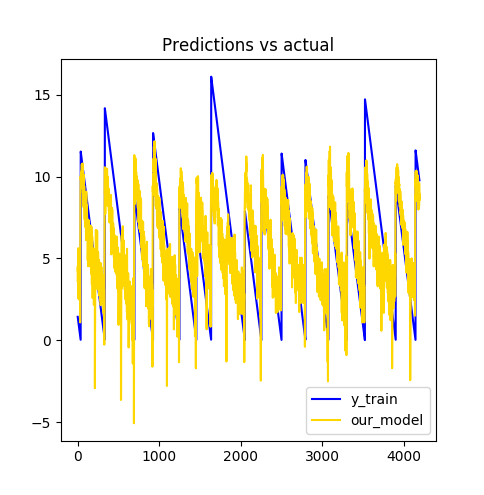
\includegraphics[width=1\linewidth]{pictures/linear_regression_24f.png}
	\caption{Linear Regression, 24 features, \texttt{time\textunderscore to\textunderscore failure} predictions vs real values.}
	\label{fig:LR}
\end{figure}

After submitting our results to Kaggle's platform, the score of this kernel calculated by the system was \textbf{1,660}. Other attempts to improve this solution by adding more features were unsatisfactory.

%Linear Regression + 5 features (mean, std, pp, q05, q95) + 5*3 rolling windows features: 2,1076697 (pp = peak-to-peak value)
%Linear Regression + 24 features + 12*3 rolling windows features: 2,111956

\section[Second model]{Second model: Support Vector Regression on more features}
\label{3.2}
%Standard Scaler doesn't change the score
%Lasso same param.: score is worse, increment alpha/num iterations? NO
%Elastic Net same param, list of cv param : still score is worse; attempt 2, alpha set from None to 1, iterations from 1000 to 10000, tolerance from 0.0001 to 0.001 -> (1) errors, ravel() to flatten y_train; (2) array of dimension 0? deleted all the parameters to ElasticNetCV; (3) gave up; (4) on just one feature (mean) it works (3,048) NO
%Kernel Ridge alpha 1.0: still bad (2.25) -> tried to reduce the set of features (deleting: kurt, skew, q01, q99 and their abs versions) to improve degrees of freedom, got worse (2,29) NO
%Isotonic: found out it only works in 1d; tried to work only on the mean, just out of curiosity -> 3,04 (implementations of multiisotonic regression have been researched upon and studied but rely on the concepts of ordering and distances, which don't adapt well to our case of study) NO
After applying linear regression to an expanded set of features, the following choice was for us to merge the intuition of using more than the basic features while relying on the Support Vector Regression as for the na{\"i}ve solution. The same 24 features described in \ref{3.1} were used, while our exploration in this type of model was mainly focused on the choice of the kernel function (chosen through a parameter defined in the implementation of \texttt{NuSVR} inside \texttt{scikit-learn}). It must also be remembered that, as stated in the documentation, this model needs data to be previously scaled (otherwise performances decrease considerably).

The choice of the kernel function in this case is crucial: a \textit{kernel function} makes it possible to transform data from a \textit{n}-dimensional space (in our case, defined by the set of computed features) into another space with reduced dimensions, in order to find a more clear dividing margin between classes ("\textit{kernel trick}"). There are of course different choices for the kernel function: radial basis function, linear, polynomial, just to name some of them.

Results of changing the \texttt{kernel} parameter were the following, in terms of score on the training set:
\begin{itemize}
	\item \texttt{rbf} or \textit{radial basis function}, default: 2,1038;
	\item \texttt{linear}: 2,1638 (also, quite a few negative results for the submission file);
	\item \texttt{poly} or \textit{polynomial}: 2,5109861 (even more negative results).
%	\item \texttt{sigmoid}:15.932038 (wtf)
\end{itemize}

\begin{figure} [h]
	\centering
	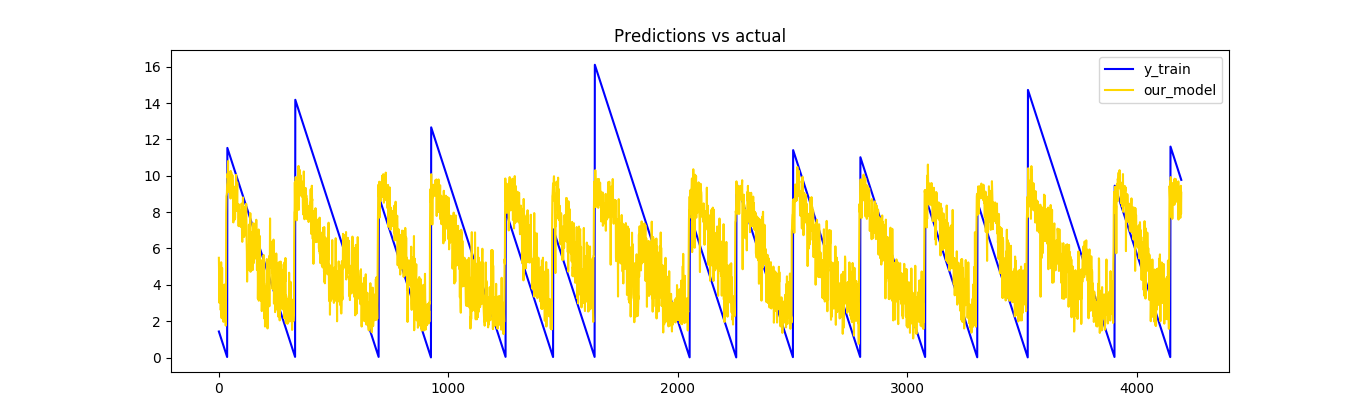
\includegraphics[width=1\linewidth]{pictures/nu_svr_24f.png}
	\caption{Support Vector Regression with \texttt{rbf}, 24 features, \texttt{time\textunderscore to\textunderscore failure} predictions vs real values.}
	\label{fig:SVR}
\end{figure}

After submitting our results to Kaggle's platform, the score of this kernel calculated by the system was \textbf{1,609}.

\section[Feature selection]{Introducing preliminary feature selection}
Due to the high dimensionality of the dataset, the computations made on it take several minutes to be completed. In order to boost performances and with the goal to improve the accuracy of the models, our next attempt was to introduce a preemptive feature selection.

\textit{Feature selection} can be seen as a pre-processing step, that works by selecting the best features on the basis of some specified tests.

\texttt{Scikit-learn} exposes some choices for this purpose, among which \texttt{SelectKBest} and \texttt{SelectPercentile} (the former removing all but the \textit{k} highest scoring features, the latter keeping the specified percentage of highest scoring features). The scoring functions available for regression purposes are \texttt{f\textunderscore regression} (being able to capture linear correlations between features) and \texttt{mutual\textunderscore info\textunderscore regression} (which underlines some more particular correlations). Our choices for the solution were to use \texttt{SelectKBest} with \texttt{mutual\textunderscore info\textunderscore regression} to select the best 10 features, to be tested afterwards with our most promising model up until now, \texttt{NuSVR} \ref{3.2}.

The 10 selected features were the ones in image \ref{fig:featsel}.

\begin{figure} [h]
	\centering
	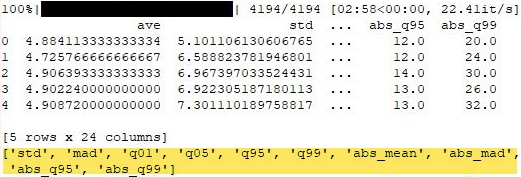
\includegraphics[width=1\linewidth]{pictures/featuresselez10_noroll.jpg}
	\caption{10 features selected from \texttt{SelectKBest}.}
	\label{fig:featsel}
\end{figure}

\begin{figure} [h]
	\centering
	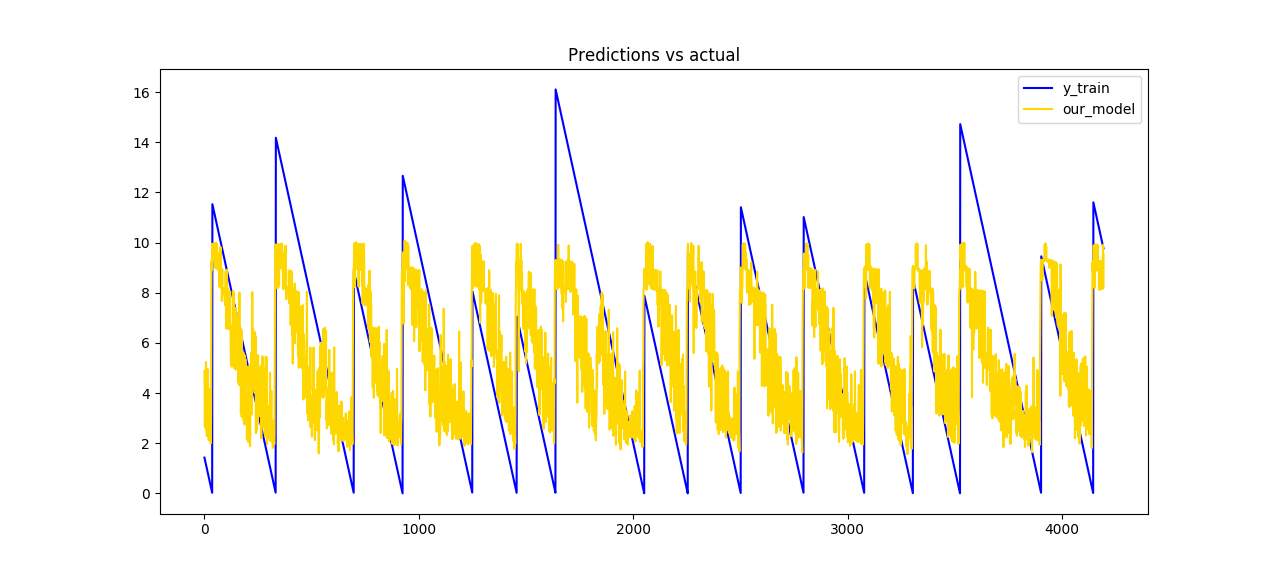
\includegraphics[width=1\linewidth]{pictures/nu_svr_featuresel10.png}
	\caption{Support Vector Regression with \texttt{rbf}, 10 selected features, \texttt{time\textunderscore to\textunderscore failure} predictions vs real values.}
	\label{fig:svrsel}
\end{figure}

The score obtained on the training set with just the above mentioned features was 2,1138, which would seem not to improve the one obtained in \ref{3.2} without feature selection; after submitting our results to Kaggle's platform though, the score of this kernel calculated by the system was \textbf{1,588}.

\section[Third model]{Third model: Neural Network Regression}
Artificial Neural Networks are computing systems inspired by biological neural networks, that learn to perform tasks by taking examples as input, generally without any task-specific rule. 
In particular, a MultiLayer Perceptron (MLP) is made at least of 3 layers: input, output and one or more hidden layers (neurons that use non-linear activation functions); thanks to the complexity, MLP can distinguish non-linearly separable data.

Implementation of MLP Regressor in \texttt{scikit-learn} has a huge set of parameters to define in order to be able to refine the model.
Our exploration focused on some of them:
\begin{itemize}
	\item \texttt{hidden\textunderscore layer\textunderscore sizes}, number of neurons in each hidden layer;
	\item \texttt{max\textunderscore iter}, maximum number of iterations;
	\item \texttt{solver}; the default is \texttt{adam}, a stochastic gradient-based optimizer that works well on large datasets, but other options are \texttt{sgd}, a stochastic gradient descent, and \texttt{lbfgs}, from the family of quasi-Newton methods;
	\item \texttt{warm\textunderscore start}, a boolean option that enables or disables initialization of the next call with the previous solution.
\end{itemize}
Various attempts on so-constructed models showed that scaling is highly recommended for performance reasons.

Picture \ref{fig:NNtries} is a synthetic representation of the different parameters settings we had the chance to test. Other than the described parameters, we also diversified the number of features used as input for the models; the results shown are computed on the training set by us, and on a portion of the test set by submitting the solutions to Kaggle's platform. What can be inferred from them is that the solution seem to work well on a medium to large-sized set of features (24 to 60) for the training set, but on a small set for the test set, and in any case on a smaller number of hidden layer neurons.

\begin{figure} [h]
	\centering
	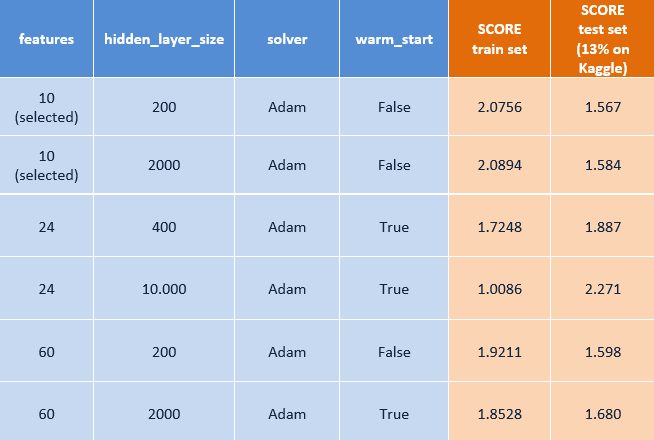
\includegraphics[width=0.9\linewidth]{pictures/table2.png}
	\caption{Attempts and results on different parameters settings.}
	\label{fig:NNtries}
\end{figure}

\bigbreak

Aside from these tries, the most successful attempt with a score of 2,0015 on the training set had the following settings:
\begin{itemize}
	\item number of features: 24;
	\item \texttt{hidden\textunderscore layer\textunderscore sizes}: 1000;
	\item \texttt{max\textunderscore iter}: 2500;
	\item \texttt{solver}: sgd;
	\item \texttt{warm\textunderscore start}: false.
\end{itemize}
Other settings in the following snippet are to print progress messages (\texttt{verbose}), to set the tolerance of the loss score between consecutive iterations (\texttt{tol}) and not to shuffle samples between iterations (\texttt{shuffle}).

\begin{lstlisting}[firstnumber=14]
from sklearn.neural_network import MLPRegressor
\end{lstlisting}

\begin{lstlisting}[firstnumber=109]
model = MLPRegressor(verbose=True, random_state=10, tol=0.000001, max_iter=2500, hidden_layer_sizes=1000, shuffle=False, solver='sgd')
\end{lstlisting}

\begin{figure} [h]
	\centering
	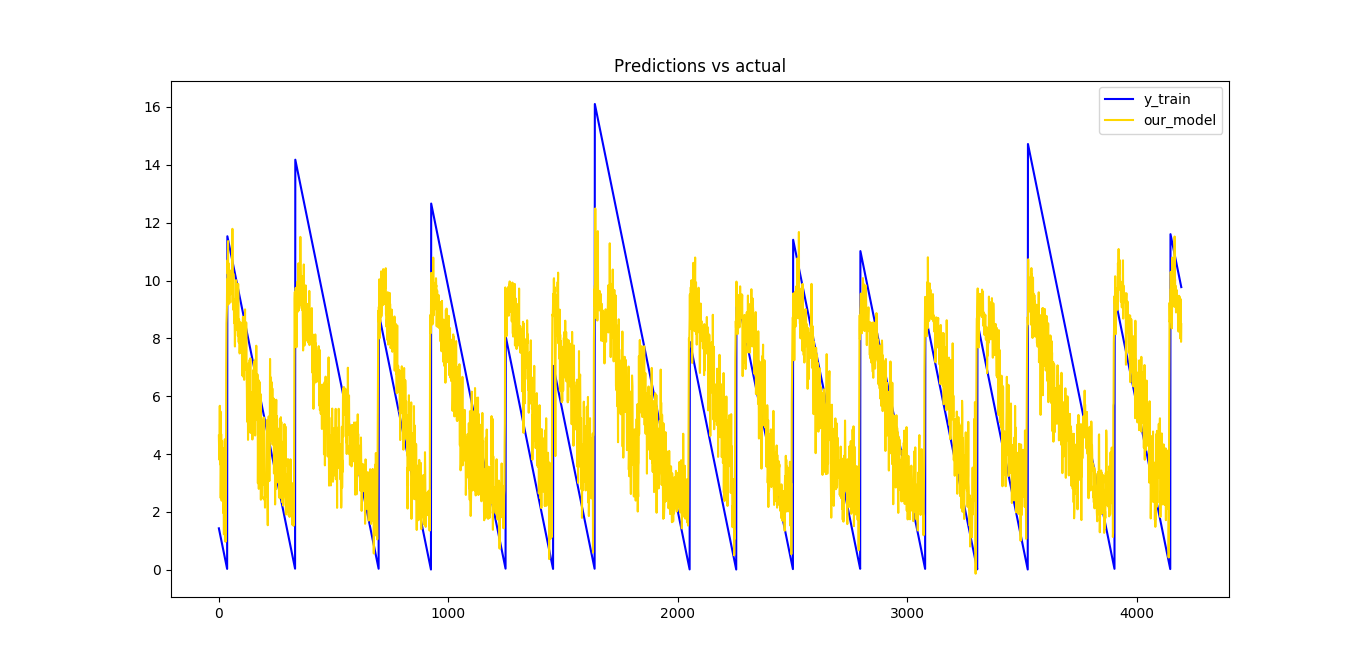
\includegraphics[width=1\linewidth]{pictures/bestnn.png}
	\caption{Best MLP Regression, \texttt{time\textunderscore to\textunderscore failure} predictions vs real values.}
	\label{fig:MLP}
\end{figure}

After submitting our results to Kaggle's platform, the score of this kernel calculated by the system was \textbf{1,540}.

\section[Overfitting]{The problem of overfitting: Gaussian Processes and Random Forests}
\textit{Gaussian Processes} are a versatile supervised learning method that aims at interpolating the observations and predicting results with some confidence intervals. Similarly to SVR, a kernel function must be specified.

Introducing the regression model based on GPs on our dataset, the results obtained were surprising to say the least: the precision score calculated on the training set was in the order of magnitude of e-10 (basically, the error didn't exist).

\begin{lstlisting}[firstnumber=14]
from sklearn.gaussian_process import GaussianProcessRegressor
\end{lstlisting}

\begin{lstlisting}[firstnumber=101]
model = GaussianProcessRegressor()
\end{lstlisting}

Indeed, the graph in \ref{fig:GP} shows that the predicted values perfectly overlap the real values of \texttt{time\textunderscore to\textunderscore failure} in the training set (notice that both have been plotted).

\begin{figure} [h]
	\centering
	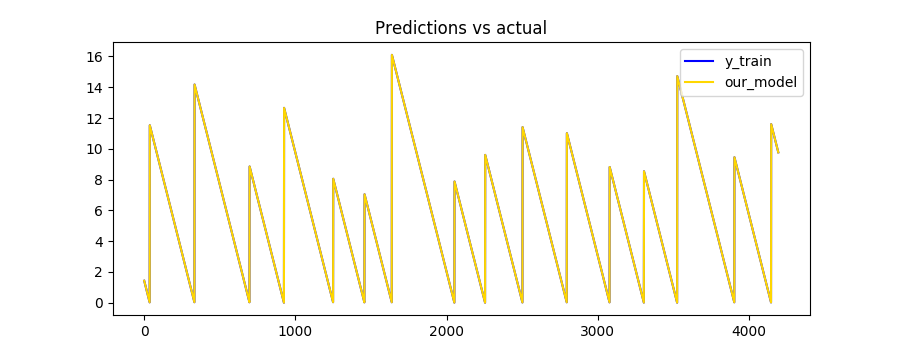
\includegraphics[width=1\linewidth]{pictures/gpr_24f.png}
	\caption{Gaussian Process Regression, 24 features, \texttt{time\textunderscore to\textunderscore failure} predictions vs real values.}
	\label{fig:GP}
\end{figure}

However, when submitting our results to Kaggle's platform tempted by the above described performances, the score of this kernel was \textbf{2,792}, showing that the built model was indeed overfitted to the training data and performed very badly on the test data.

%k-Nearest Neighbor (ave, std, pp, q01, q05, q95, q99): k=1000 -> 2,71; k=100 -> 2,44; k=20 -> 2,16; k=5 -> 1,94 (submitted: 2,024, overfitting).
%radius-Nearest Neighbor (ave, std, pp, q01, q05, q95, q99): r=5.0 -> 2,17083; r=1.5 -> 1,58 (radius too short, some values don't have neighbors within the boundaries, e.g. our "good" outliers, thus don't have predictions); r=3.5 -> 2,1094 ?

%Gradient Boosting Regression (alpha 0.95, n_estimators 230): >4, dumped NO

\bigbreak

Almost the same conclusion can be drawn for the \textit{Random Forest Regressor} (and its even more random evolution, \textit{Estremely Randomized Trees Regressor}). These are ensemble methods based on decision trees, whose purpose is to combine predictions of several estimators, doing so by building them independently, then averaging the predictions and obtaining a single base estimator with reduced variance and improved robustness.

The mechanism followed by Random Forests is to build a tree by splitting nodes according to the best split among a random subset of features; this randomness gives the model a decrease in variance with respect to a single non-random tree, that instead chooses the split out of all features. In addition, in Extremely Randomized Trees randomness is used also to select the thresholds that generate the splits.

Implementation of \texttt{RandomForestRegressor} available in \texttt{scikit-learn} takes several parameters as input, among which \texttt{n\textunderscore estimators}, that enables to specify the number of trees in the forest (the larger, the better, but the more intense will be the computation), and \texttt{criterion}, the function measuring the quality of a split (the default is \texttt{MSE}, which fits well to our situation).

\begin{lstlisting}[firstnumber=14]
from sklearn.ensemble import RandomForestRegressor
\end{lstlisting}

\begin{lstlisting}[firstnumber=115]
model = RandomForestRegressor(n_estimators=10000)
model.fit(X_train, y_train.values.flatten())
\end{lstlisting}

\begin{figure} [h]
	\centering
	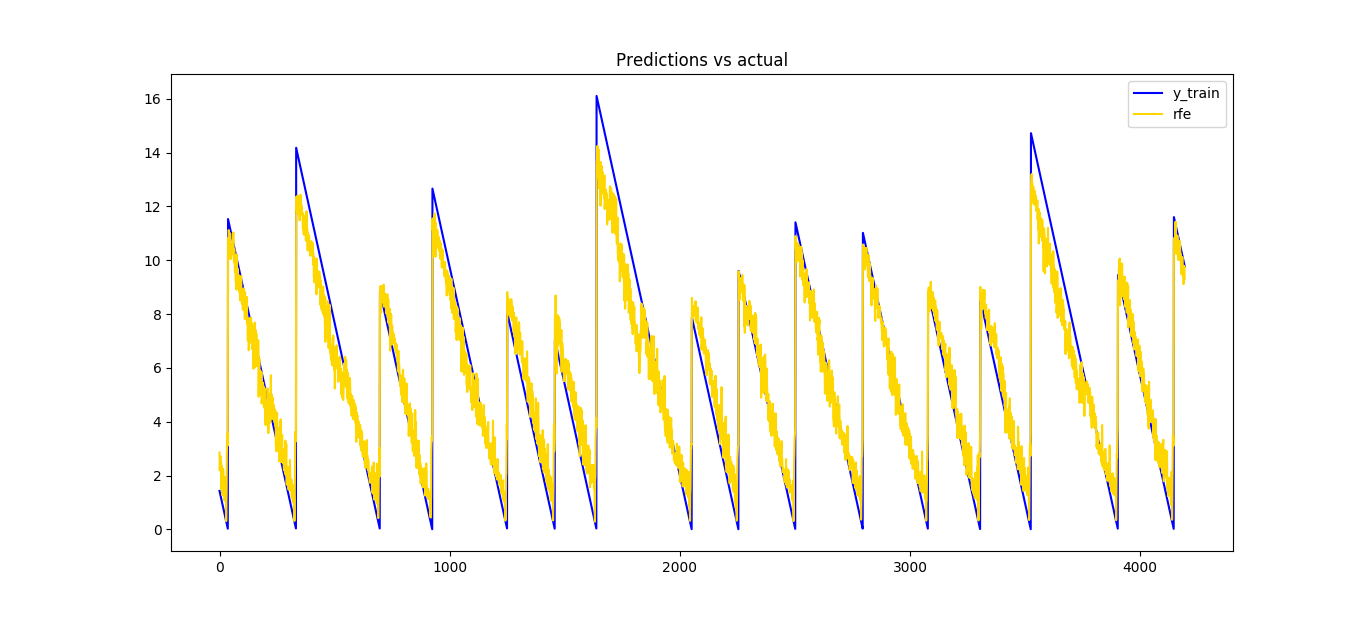
\includegraphics[width=1\linewidth]{pictures/randomforest10000.png}
	\caption{Random Forest Regression, 24 features, 10.000 iterations, \texttt{time\textunderscore to\textunderscore failure} predictions vs real values.}
	\label{fig:RF10000}
\end{figure}

Results obtained by computing the score on the available data were very encouraging: only 0,8146 for the training set while using 1000 estimators, and down to 0,7785 with 10000. After submitting our results to Kaggle's platform, though, the score of this kernel (the best case obtained) calculated by the system was \textbf{1,687}. Even if much better than GPs' results on test data, the score does not reflect the improvement obtained on the training set, showing also in this case that these more advanced models can be very precise in the building phase, but are prone to overfitting. A further development of this solution could perhaps be obtained through a better, more in-depth knowledge of the setting parameters, which was beyond the purpose of this exploring project activity.
%Random Forest Regressor (n_estimators 200): 0,816861, submitted: 1,742; n_estimators 250 -> 0,81821; n_estimators 1000 -> 05; n_estimators 100000 ? + other results